\chapter{Design}
\thispagestyle{main} % Needed for Footer and Header on Chapterpage
This chapter outlines the design of the Bazo Virtual Machine and all other components on given requirements and restrictions based on the previous work this project is based on. Furthermore trade-offs regarding different virtual machine implementations are discussed. Figure \ref{vmexecutioncycle} shows all components in one single diagram. All components and entities are described in detail in the following sections.

\begin{figure}[H]
	\begin{center}
	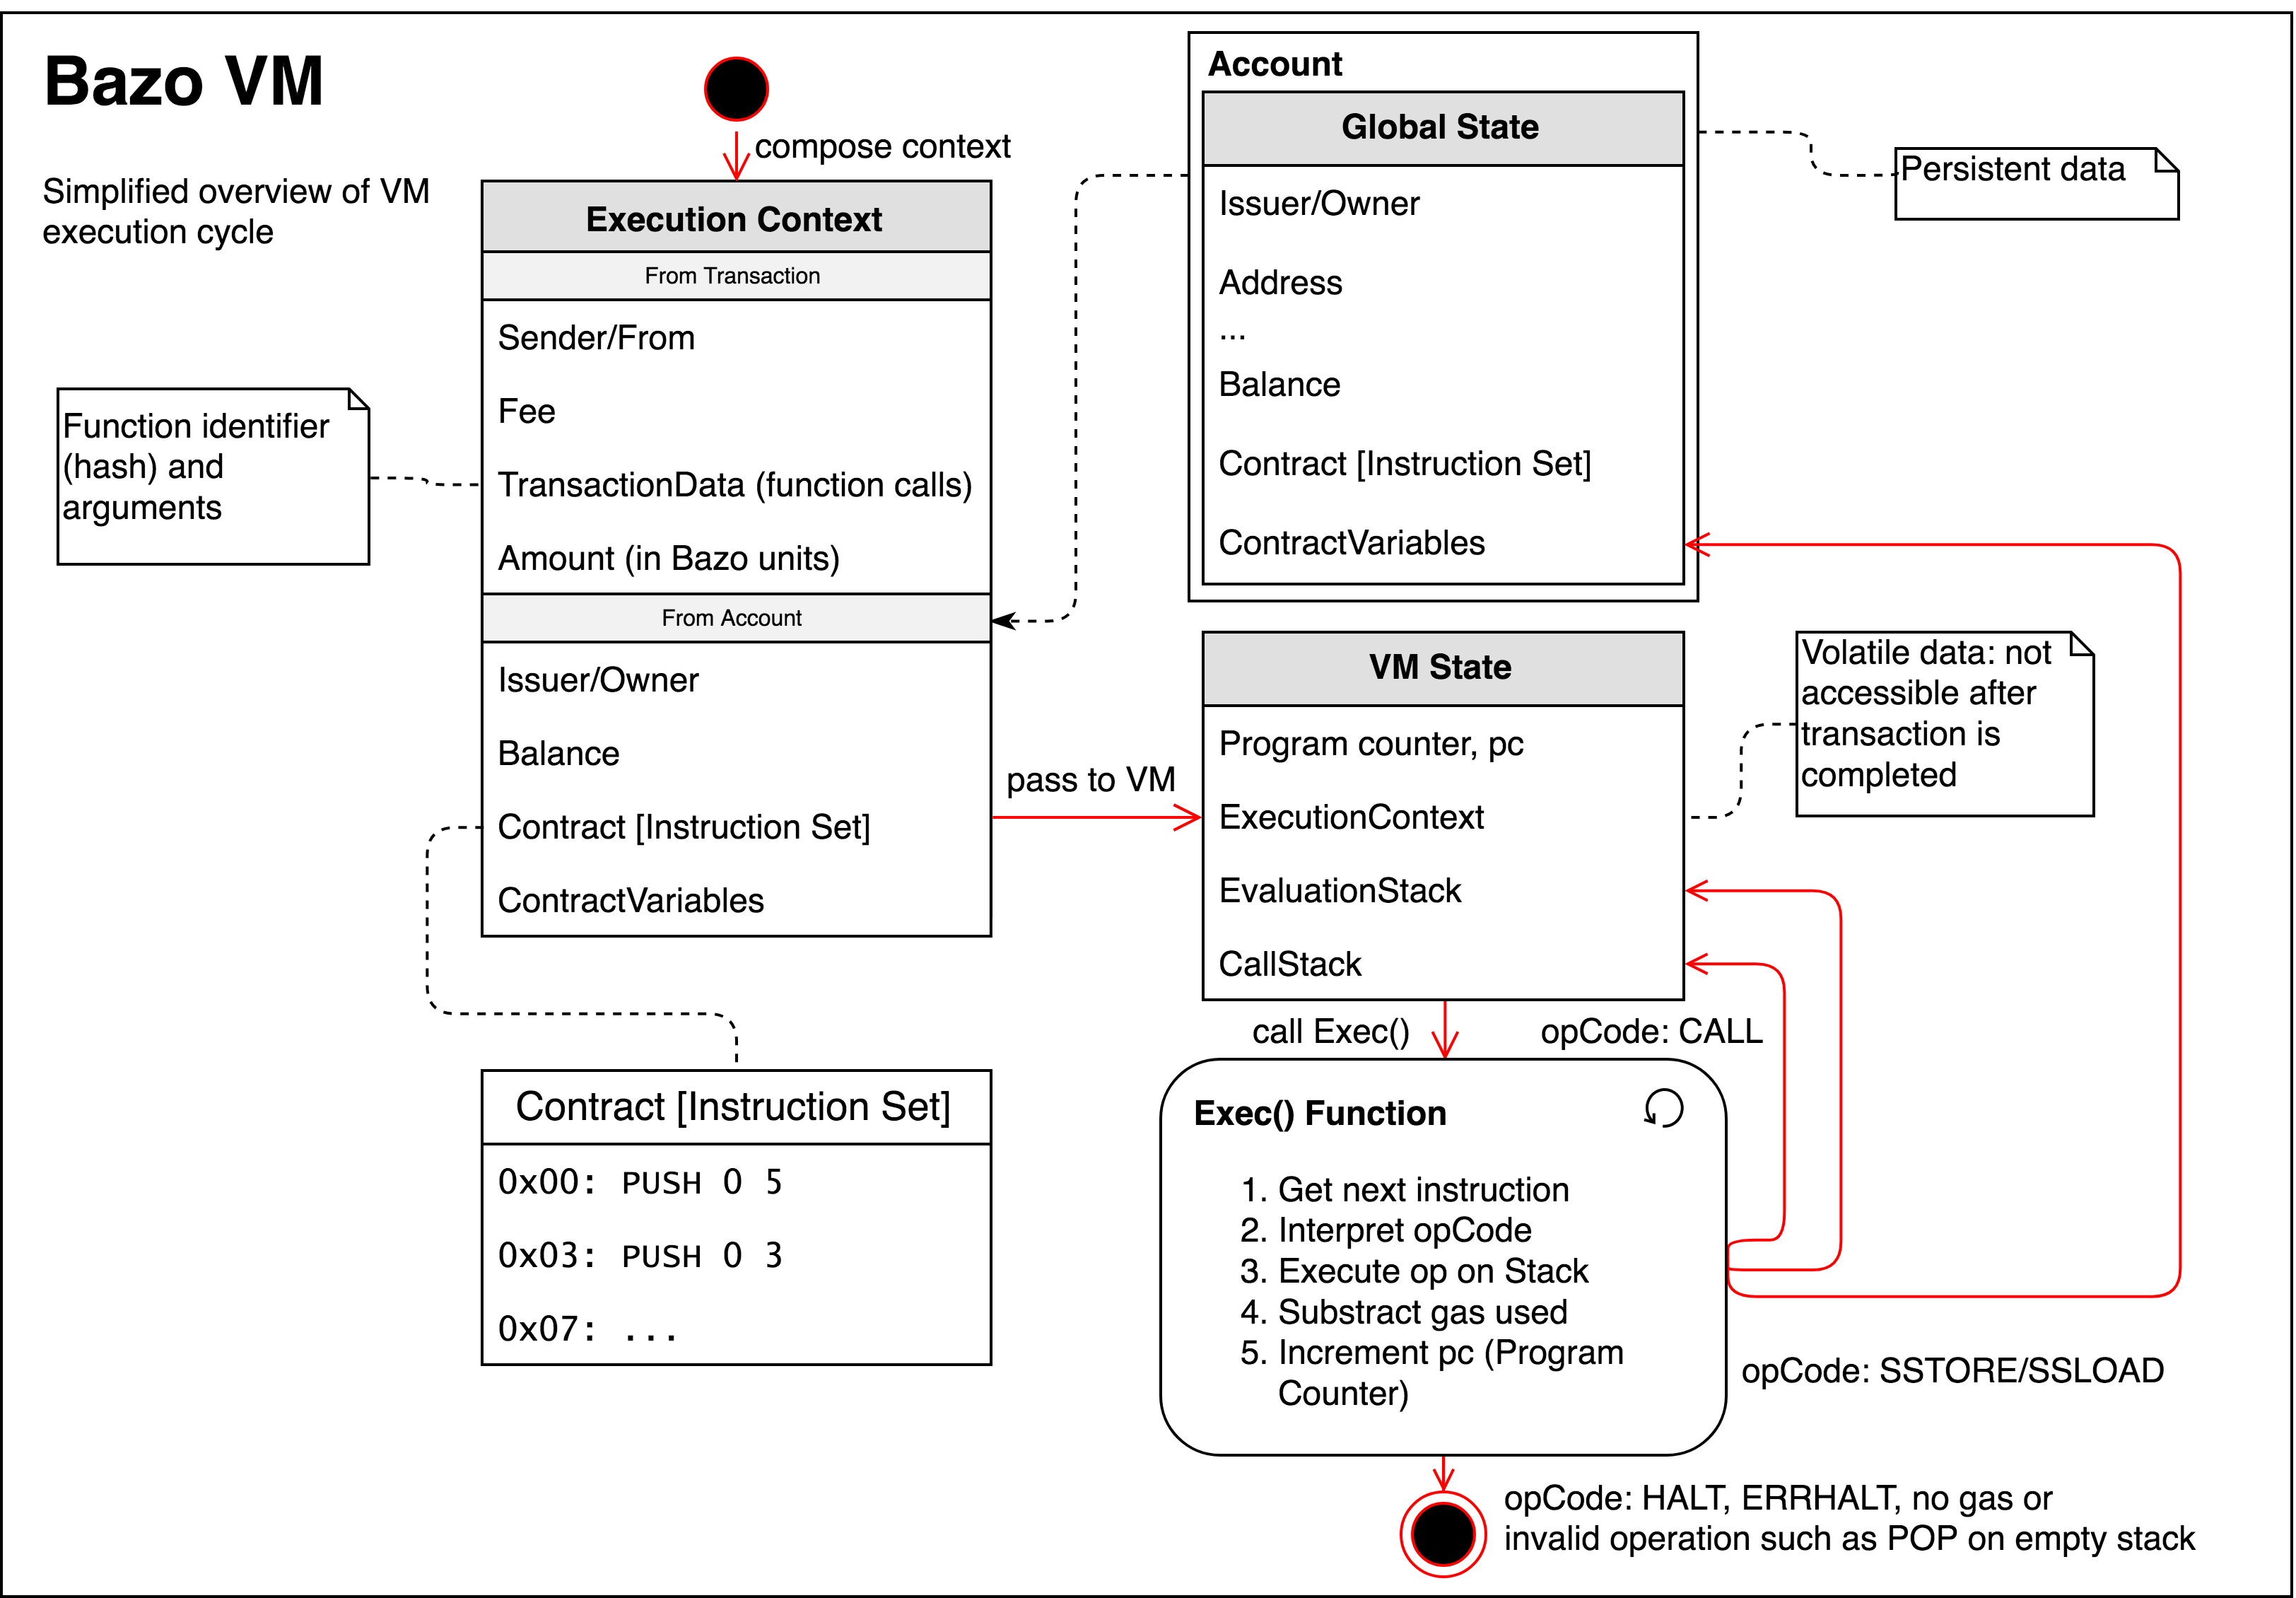
\includegraphics[width=\textwidth]{./images/execution-cycle}
	\caption{Virtual machine execution cycle}
	\label{vmexecutioncycle}
	\end{center}
\end{figure}

\section{From contract creation to the effects of its execution}
\subsection{Contract creation}
A user creates a contract via the client and it's command line interface. There he provides the necessary parameters which include the code of the contract and sends the transaction to the miner. The miner then validates the incoming transaction and creates an account according to the provided parameter on his heap memory, see section \ref{accounts} for further information about accounts. It also broadcasts the new transaction to the other miners, which then act accordingly.

\subsection{Execution of a contract method}
A user again creates a new transaction, see chapter  to call a contract. He provides the necessary parameters and the hash of the function he wants to call as parameter of the new transaction. This new transaction again is transmitted to the miner, as he sees the type of the transaction and that it has parameters in the data field it will find the called contract and execute it's code according to the provided parameters in the data field. Now the user can check the changed properties on the blockchain. 
\pagebreak

\section{Virtual machine}
There are two types of virtual machines. On the one hand there are register based virtual machines. Examples of register based virtual machines are the Lua VM and the Dalvik VM. On the other there are stack based virtual machines. The Java Virtual Machine and the .NET CLR were both stack based virtual machines. 
\begin{description}
  \item[Register based] The data structure of where the operands are stored is based on registers of the CPU, therefore the instructions need to contain the addresses (registers) of the operands. This leads to longer instructions. Figure \ref{register vm} shows how adding two number works on a register based virtual machine. \cite{stackvsregistervm} The instruction is \mintinline{tasm}{ADD R1 R3 R2}.
  \begin{figure}[H]
	\begin{center}
	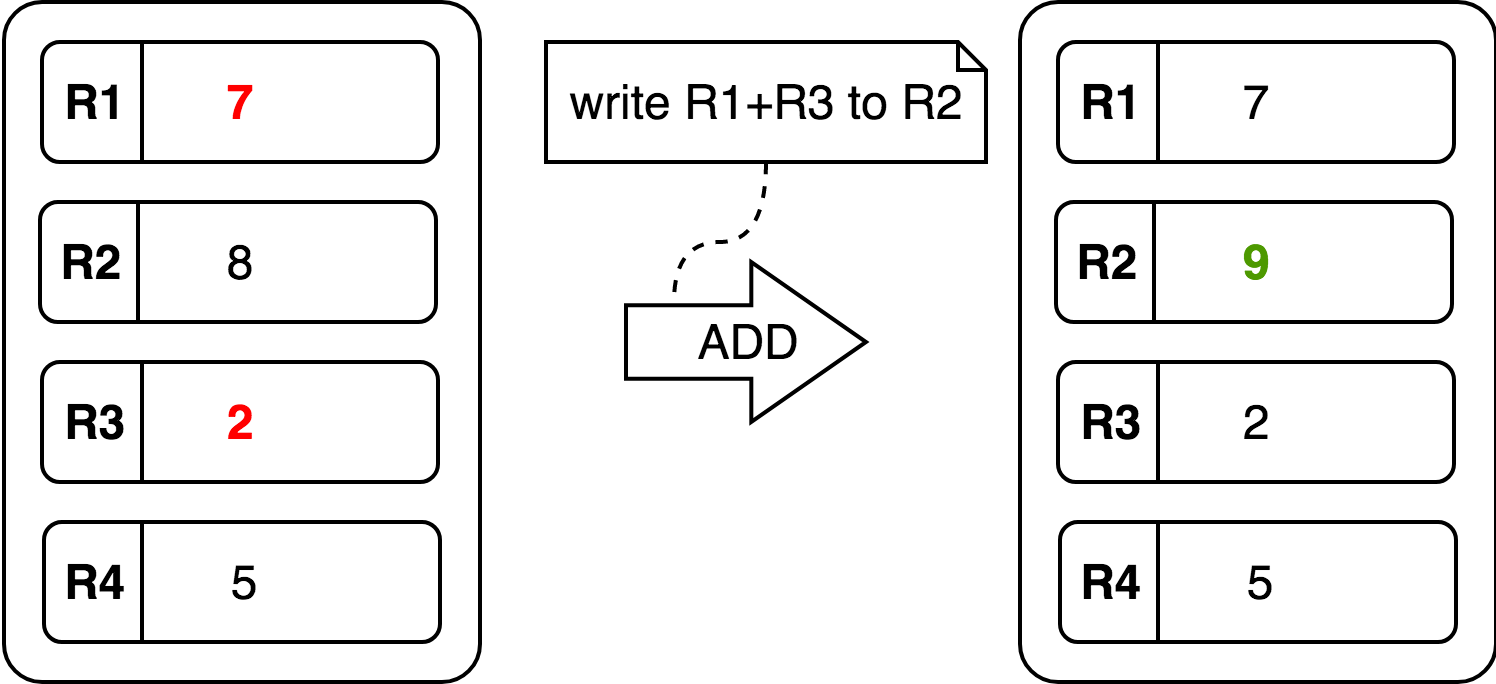
\includegraphics[width=0.5\textwidth]{./images/register-example}
	\caption{Register based virtual machine}
	\label{register vm}
	\end{center}
  \end{figure}
  
  \item[Stack based] A stack based virtual machine is based on a LIFO (last in, first out) stack. Operations are carried out by popping and pushing back results on the stack. The main advantage is a stack pointer that implicitly addresses the operands, which means that no addresses are passed in instructions. The instructions code is longer since \mintinline{tasm}{POP} and \mintinline{tasm}{PUSH} instructions have to be included to retrieve and store the operands. \cite{stackvsregistervm} The instruction to add two numbers as shown in figure \ref{stack vm} are: 
  \begin{figure}[thp]%
    \centering
	\begin{minipage}{0.4\textwidth}
  \begin{minted}	[
	frame=lines,
	framesep=2mm,
	baselinestretch=1.2,
	fontsize=\footnotesize,
	linenos
	]
	{tasm}
	POP
	POP
	ADD
	PUSH
  \end{minted}
  \end{minipage}
  \end{figure}
  \begin{figure}[H]
	\begin{center}
	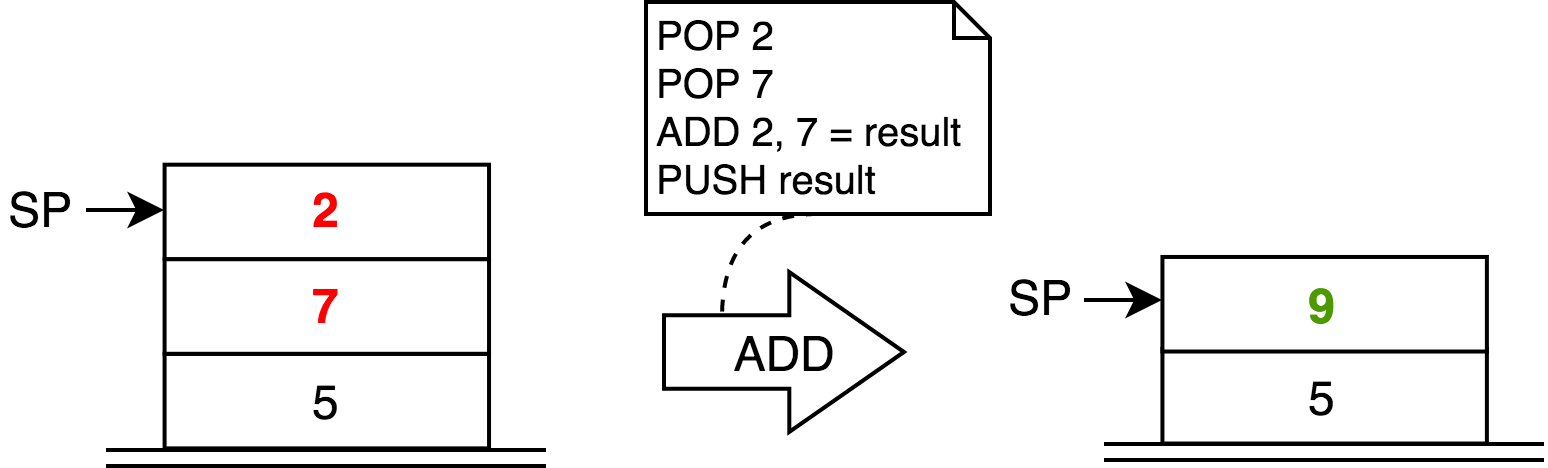
\includegraphics[width=0.6\textwidth]{./images/stack-example}
	\caption{Stack based virtual machine}
	\label{stack vm}
	\end{center}
  \end{figure}
\end{description}

Despite the register based virtual machine having advantages such as more possibilities for optimizations and having no overhead from pushing and popping, over a stack based virtual machine we decided to implement a stack based virtual machine. This decision was most influenced by the implementation of related projects, namely Ethereum and NEO, on which we have oriented ourselves.

\subsection{VM Execution cycle}
This section describes the \mintinline{go}{Exec()} function shown in figure \ref{vmexecutioncycle}.
Precondition that the VM execution cycle is started is, that the transaction must be sent to a smart contract account and the transaction data is not empty. If these preconditions can be fulfilled, the vm execution cycle is started by the miner.

The starting point for the execution cycle of the virtual machine is a set of instructions and an incrementing counter, called the program counter, which points to the instruction that is executed next.

The instruction cycle can be divided into three steps which are repeated over and over again until an invalid instruction occurs, the execution is halted by an instruction itself or the program counter is out of bounds of the instruction set. All this steps are handled in the \mintinline{go}{Exec()} function. This are the three steps:
\begin{description}
  \item[Fetch] The instruction of the instruction code where the program counter points to is fetched. After it is fetched, the program counter is increased.
  \item[Decode] The instruction is interpreted by the decoder. The decoder matches the instructions with pre-defined opcodes, which can be interpreted by the execute function.
  \item[Execute] The instruction is executed on the stack according to the opcode. There are opcodes for arithmetic operations, e.g. \mintinline{yaml}{ADD, MOD, SUB}, for flow operations e.g. \mintinline{yaml}{JMP, CALL, RET} which are allowed to change the program counter and therefore move back and forward in the instruction set, cryptographic operations, such as \mintinline{yaml}{SHA3, CHECKSIG} and context operations, e.g. \mintinline{yaml}{ADDRESS, ISSUER, CALLER, CALLDATA} that can be used to push context data composed from the transaction and the receiver account to the stack and opcodes for storing and loading state variables \mintinline{yaml}{SSTORE, SLOAD}. All implemented opcodes are listed in table \ref{opcodes-list}.
\end{description}
\section{Miner}

\subsection{Transaction Types} \label{transactionTypes}

\cite{ba_client}

\begin{figure}[thp]%
    \centering
	\begin{minipage}{0.4\textwidth}
	\begin{minted}
	[
	frame=lines,
	framesep=2mm,
	baselinestretch=1.2,
	fontsize=\footnotesize,
	linenos
	]
	{go}
	type FundsTx struct {
		Header byte
		Amount uint64
		Fee    uint64
		TxCnt  uint32
		From   [32]byte
		To     [32]byte
		Sig1   [64]byte
		Sig2   [64]byte
		Data   []byte
	}
	\end{minted}
\end{minipage}
\end{figure}

\subsection{Accounts} \label{accounts}
Accounts are the result of processing an account transaction. They are object on the heap of the miner. The bazo miner already had the transaction type to create accounts by design.

\subsubsection{Externally owned accounts}
Externally owned accounts are accounts that are owned by the person which has access to the combination of the public and private key. Having both the person is able to execute transaction subtracting the balance. The creation of externally owned accounts was already given by the previous thesis by Livio Sgier.

\subsubsection{Smart contract accounts}
Smart contracts accounts are created and owned by externally owned accounts. Smart contracts accounts have two additional fields, which were added to the account creation transaction.

\begin{description}
  \item[Contract] This field contains the smart contract.
  \item[ContractVariables] This field contains the state variables that can be altered by contract functions.
\end{description}

\section{Smart contracts}
Smart contracts are programs that are stored on the blockchain. A smart contract consists of an ABI (application binary interface) and one or more callable functions. Smart contracts are deployed through a transaction (AccTx). Calling a certain function is also made through a transaction (FundsTx). When someone wants to call a certain function in a smart contract, a special transaction to the public address of the smart contract is executed. The transaction contains an identifier in a designated data field, so the ABI can match the identifier with the function the caller wants to execute. Arguments passed to that function are also transmitted in that field. Since a transaction is processed simultaneously on all nodes of the network, all functions have to be deterministic.

\subsection{Coding smart contracts}
Smart contracts for the NEO blockchain can be coded in C\#, Java, Kotlin, F\# or Python. There are different ways to create an Ethereum smart contract. There are different high-level programming languages that can be compiled to Ethereum byte code. Solidity is being developed by the Ethereum community and is the industry standard. Solidity is heavily inspired by JavaScript with the idea to attract JavaScript developers to write smart contracts.

\subsubsection{Sample smart contact in Solidity}
%\begin{lstlisting}[caption={Solidity contract},captionpos=b,label={lst:dialogex}]
	
%\end{lstlisting}
\begin{figure}[thp]%
    \centering
	\begin{minipage}{0.5\textwidth}
\begin{minted}
[
	frame=lines,
	framesep=2mm,
	baselinestretch=1.2,
	fontsize=\footnotesize,
	linenos
]
{javascript}
contract MyFirstContract {
  uint myData; //State variable

  function set(uint x) public {
    myData = x;
  }

  function add(uint amount) public {
    myData += amount;
  }

  function sub(uint amount) public {
    myData -= amount;
  }

  function get() public constant returns (uint) {
    return myData;
  }
}
\end{minted}
\end{minipage}
\end{figure}

This contract has the state variable myData. Calling the function set() with an uint parameter sets the variable. Calling the function add or sub allows the transaction sender to either add or subtract a certain amount from that variable. In order to call a function a transaction must be executed.
\pagebreak

\subsubsection{Sample smart contract in bazo-vm byte code instructions}
Compiled Smart Contract with ABI would look like this:
\begin{figure}[thp]%
    \centering
	\begin{minipage}{0.7\textwidth}
\begin{minted}
[
	frame=lines,
	framesep=2mm,
	baselinestretch=1.2,
	fontsize=\footnotesize,
	linenos
]
{yaml}
CALLDATA        # Puts the arguments passed to the smart contract
                # and the function hash on top of stack
# ABI:
DUP
PUSH set
EQ
JMPIF set

DUP
PUSH add
EQ
JMPIF add

DUP
PUSH sub
EQ
JMPIF sub

HALT

:set            # set function
SSTORE myData   # stores the variable in ContractVariables
HALT

:add            # add function
POP
SLOAD myData    # loads the variable and puts a local copy on the stack
ADD
SSTORE myData   # overwrites the variable in ContractVariables
HALT

:sub            # sub function
...	
\end{minted}
\end{minipage}
\end{figure}

\section{Execution context}
With data coming from the transaction, the account and the miner the Execution Context is composed. The Execution Context contains all the data needed to start the execution cycle. Every field is needed and/or can be used by the virtual machine. We use the pattern parameterize from above and encapsulate copies of all the variables we want to access in a context object.

Providing specific byte code instructions that put the value of a certain field on the top of the stack smart contract, functions that for instance can only be called by the owner of the smart contract account or functions that only can be executed if the balance is enough can be created.

\subsection{Data from transaction}
\begin{description}
  \item[Sender] The sender field shows the transactions sender public address.
  \item[Fee] The maximum price the transaction can cost.
  \item[TransactionData] This field contains the identifier to the function the sender wants to call on a certain smart contract and its arguments. In order to identify the function and still being able to override functions and enable polymorphism, the identifier is a hash build from the function signature (name and parameters).
  \item[Amount] This field shows the amount of bazo units send in this transaction.
\end{description}

\subsection{Data from account}
\begin{description}
  \item[Issuer/Owner] This field contains the public address of the account owner.
  \item[Balance] This field contains the amount of coins this account owns.
  \item[Contract] This field is the smart contract itself and contains the byte code. The datatype is \mintinline{yaml}{[]byte}, so it can easily be packed into a transaction field.
  \item[ContractVariables] This field contains the state variables that are changed by executing transactions.
\end{description}

\subsection{Data from miner}
\begin{description}
  \item[Block header] This field is needed for block number/hash
\end{description}

\section{Fee}
Running a node in the network carries costs and the node operators want to be compensated. The fee is expressed in the smallest unit of bazo coins available. The cost of execution vary since depending on the complexity of the function the amount of time which the whole network is busy processing differs. Ethereum calculates the cost depending on which instructions (such as ADD known from assembler) are used. In Ethereum and Neo this fee is called gas. Bitcoin calculates the cost depending on the size of the transaction. We combine both concepts with the goal of simplifying the calculation of the execution fee.

The fee is also a way to secure the network. As mentioned before the execution must be deterministic. Using a JUMP instruction (changing the program counter of the execution) a smart contract creator could develop a smart contract function containing an endless-loop, which then he could call, causing the network to jam and not accepting new transactions because the execution doesn't come to an end. With the introduction of gas subtracted with every instruction once no more gas is available the processing of the transaction is aborted.